\section{Análisis Experimental}

\begin{figure}
  \begin{center}
  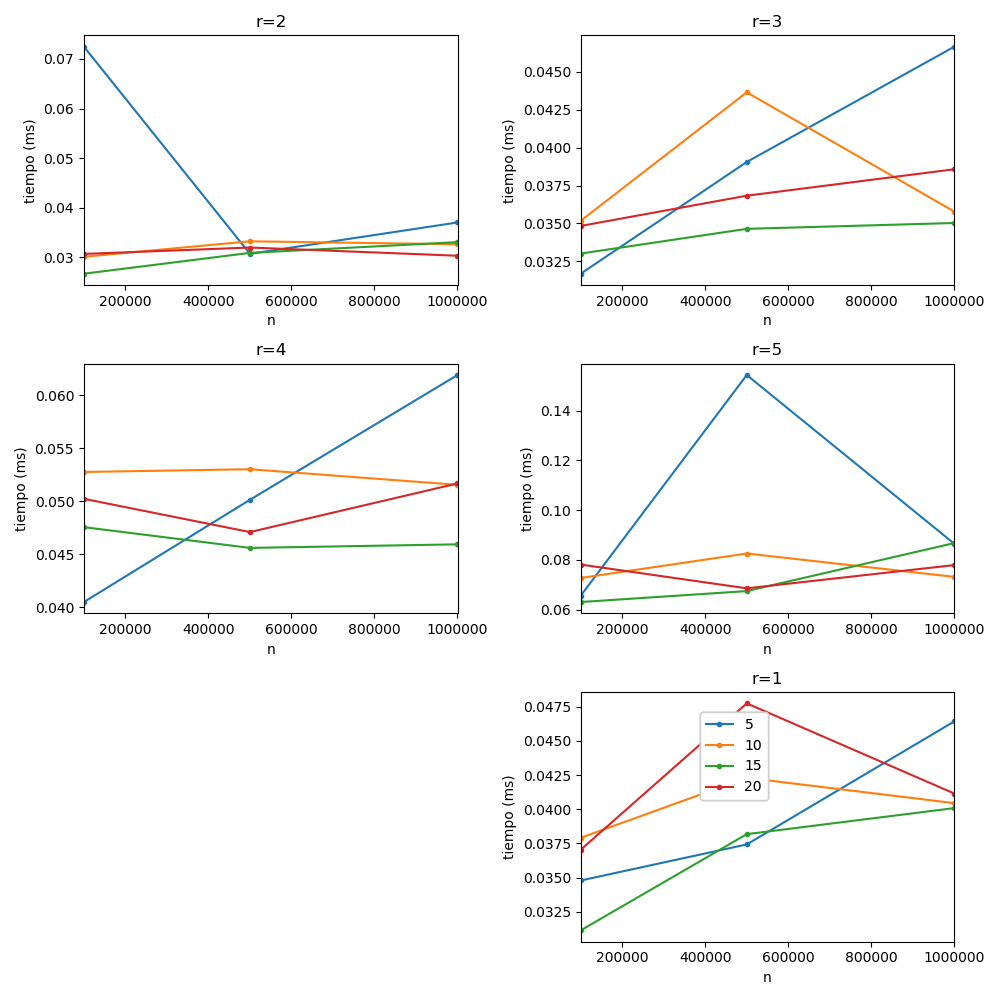
\includegraphics[width=\textwidth]{buscar_pos_n}
  \caption{Tiempo de búsqueda (positiva)
    según n, para distintos valores de r y k.}
  \label{fig:buscar-pos}
  \end{center}
\end{figure}


\begin{figure}
  \begin{center}
  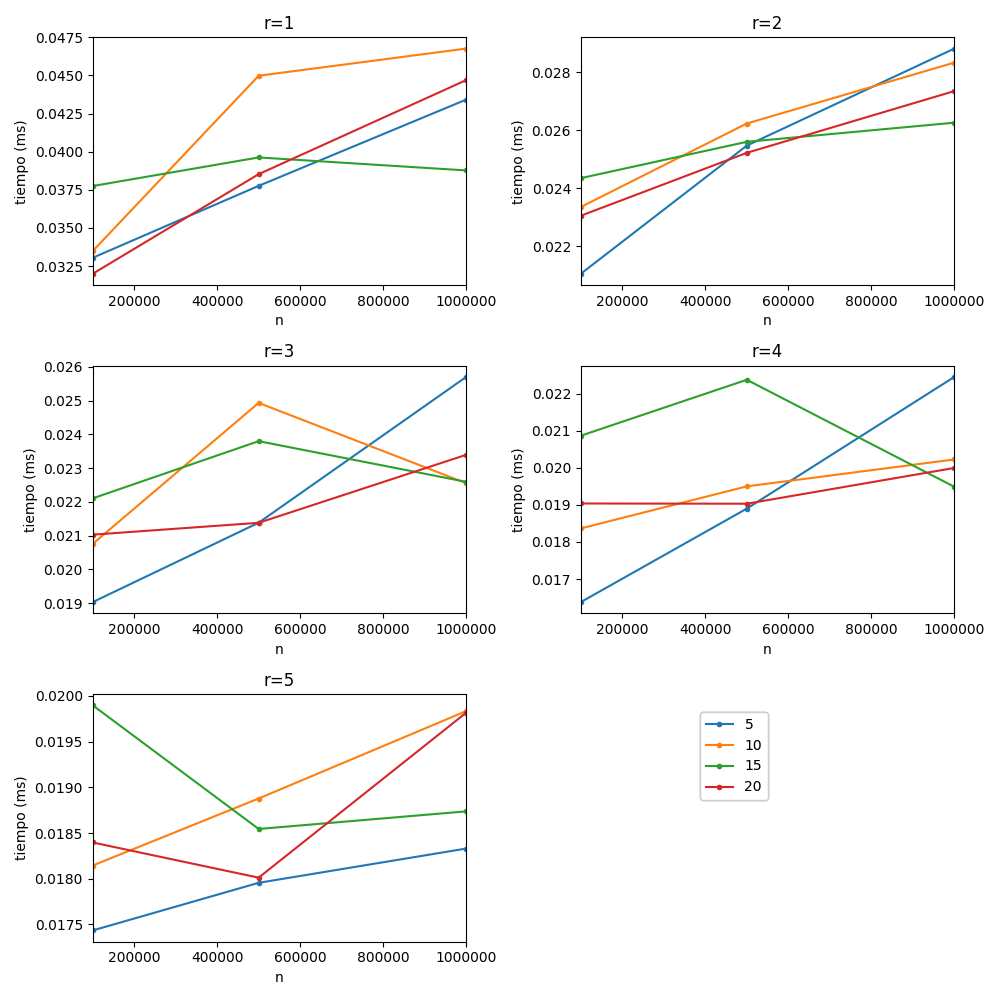
\includegraphics[width=\textwidth]{buscar_neg_n}
  \caption{Tiempo de búsqueda (negativa)
    según n, para distintos valores de r y k.}
  \label{fig:buscar-neg}
  \end{center}
\end{figure}

En las figuras \ref{fig:buscar-pos} y \ref{fig:buscar-neg} podemos
ver un crecimiento ligeramente cercano al logarítmico (que con tan solo 3
valores\footnote{Como se indica en la consigna} para \(n\) es difícil
distinguir).

La diferencia para distintos r (dado un k) se observa en la figura
\ref{fig:buscar}, y en todos los casos podemos observar que el árbol
con mayor r tiene un mejor rendimiento para las búsquedas tanto positivas como
negativas.

\begin{figure}
  \begin{center}
  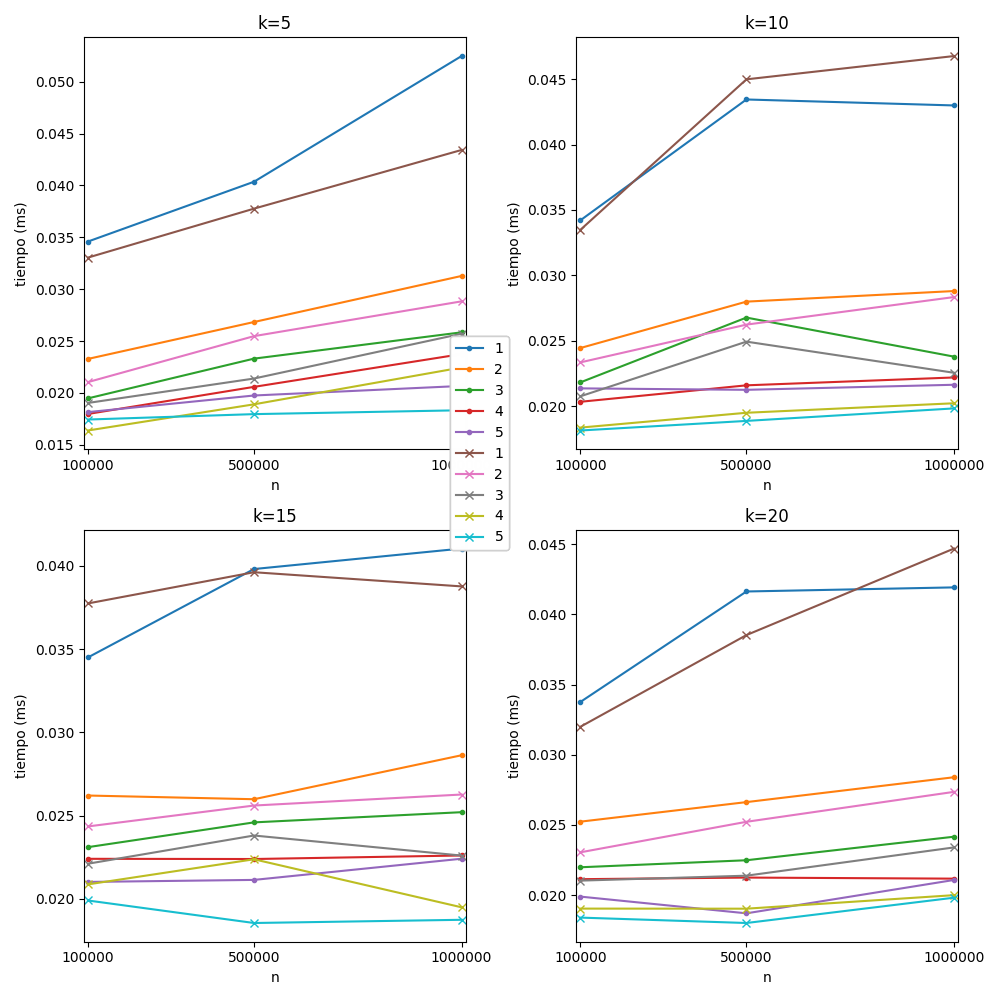
\includegraphics[width=\textwidth]{buscar_n}
  \caption{Tiempo de búsqueda (positiva y negativa)
    según n, para distintos valores de r y k.}
  \label{fig:buscar}
  \end{center}
\end{figure}

Esto se alinea con el desarrollo teórico, ya que \(r\) indica el factor de
ramificación, y cuanto mayor sea menos niveles debe recorrer hasta completar la
búsqueda.

Se observa una pequeña superioridad de las búsquedas negativas ante las positivas,
pero la diferencia no es significativa.

\begin{figure}
  \begin{center}
  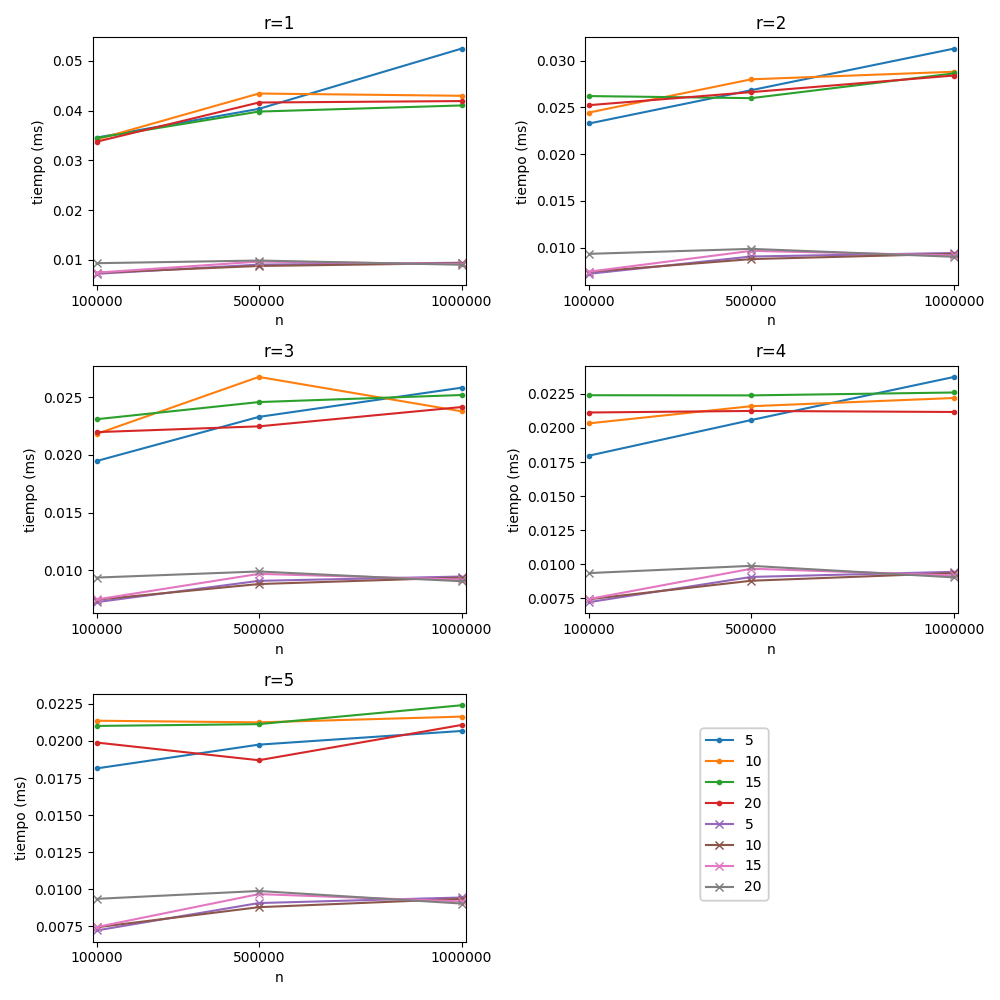
\includegraphics[width=\textwidth]{buscar_pos_kd_n}
  \caption{Tiempo de búsqueda (positiva)
    según n, para distintos valores de r y k, comparado con el árbol kd.}
  \label{fig:pos-kd}
  \end{center}
\end{figure}


\begin{figure}
  \begin{center}
  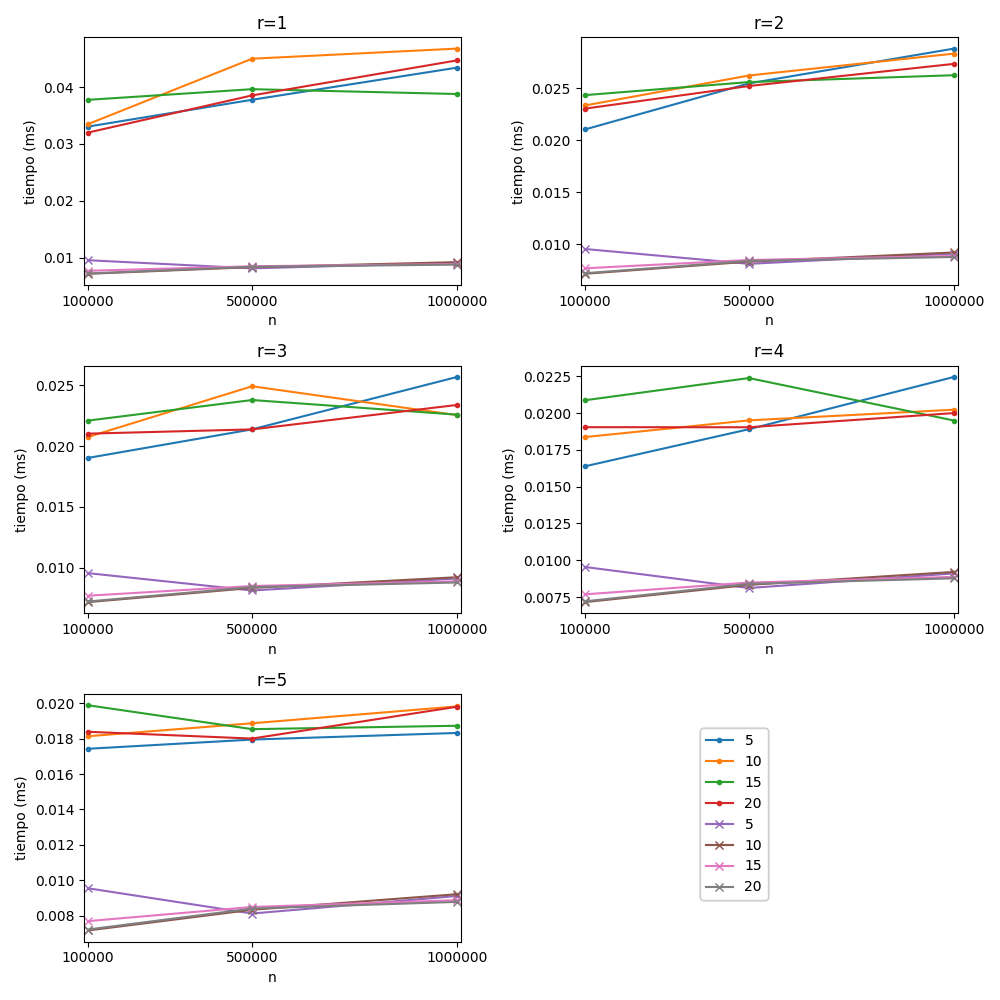
\includegraphics[width=\textwidth]{buscar_neg_kd_n}
  \caption{Tiempo de búsqueda (negativa)
    según n, para distintos valores de r y k, comparado con el árbol kd.}
  \label{fig:neg-kd}
  \end{center}
\end{figure}


En las figuras \ref{fig:pos-kd} y \ref{fig:neg-kd} podemos observar
una clara superioridad del árbol kd de búsqueda, logrando sus
búsquedas siempre por debajo de los 0.010ms, y esto se mantiene para
todo k y todo r. Ente los árboles kdr se observa variabilidad pero no
es significativa. Aún más, la creación de árboles
(fig. \ref{fig:armado}) muestra que la creación de arboles kd es
también superior, lo que es de esperar por la mayor complejidad del
algoritmos al tener que comparar r medianas.


\begin{figure}
  \begin{center}
  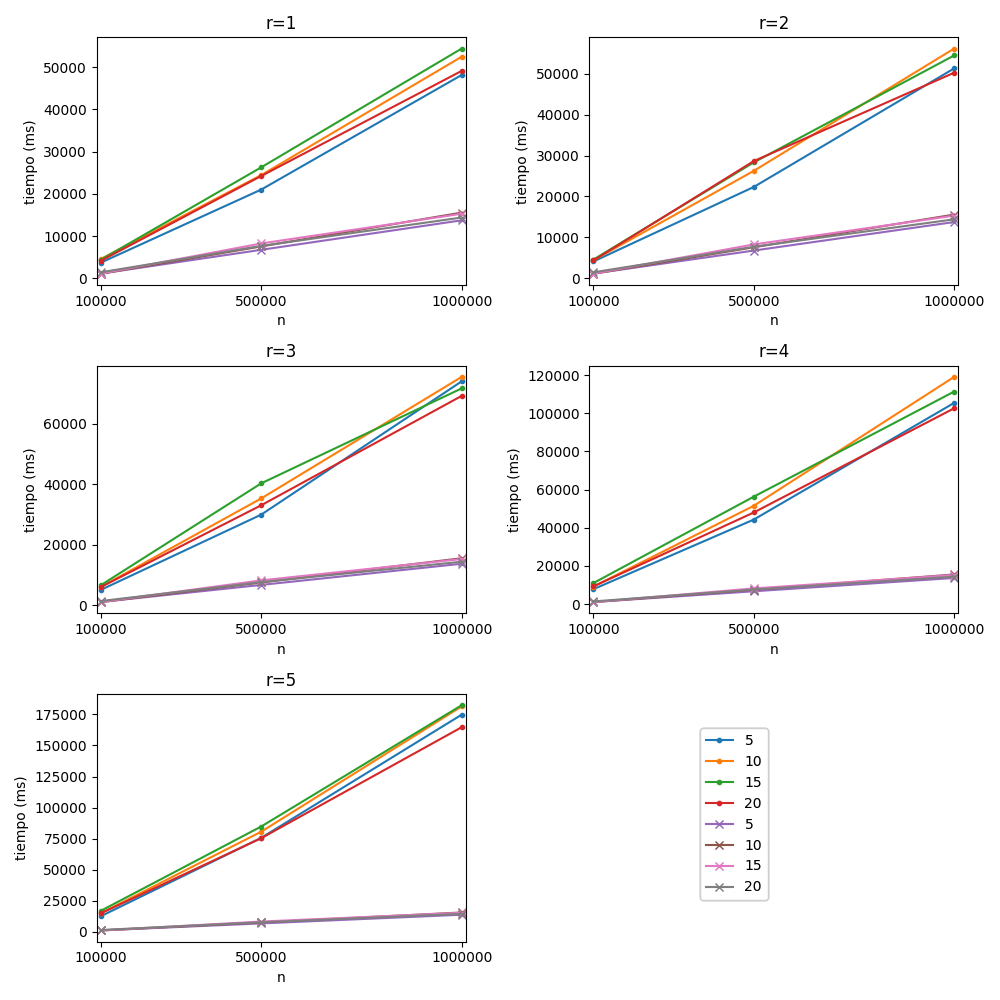
\includegraphics[width=\textwidth]{armado_n}
  \caption{Tiempo de creación de los arboles kd y kdr
    según n, para distintos valores de r y k.}
  \label{fig:armado}
  \end{center}
\end{figure}

\section{Conclusiones}
La hipótesis del proyecto plantea si resulta más eficiente la
búsqueda al particionar el subconjunto de puntos en más de una
dimensión.
Fue necesario analizar empíricamente ambos algoritmos, para poder
concluir qué sucede eventualmente.
Podemos apreciar, luego del análisis, que la búsqueda KDR,
mas allá de su aparente ventaja por reducir el número de niveles en la
búsqueda (particionando al conjunto en \(2^r\) subconjuntos), no logra
mejorar los tiempos que da el árbol kd tradicional,
y su construcción es además aún peor que el kd.

De todas formas, creemos que el proyecto fue muy productivo para poner
en práctica los conceptos aprendidos en clase, desde escribir el
código del algoritmo,  
analizar el orden de tiempo de ejecución, hasta ejecutar pruebas y
simulaciones.
Algunas obstáculos que se nos presentaron fueron la función
matches\_criteria, que inicialmente presentaba orden exponencial, lo
cual aumentaba el orden de tiempo de ejecución y hacía aún mayor la
brecha entre ambos,
como también, realizar las simulaciones, que resultaron llevar más
tiempo de lo dimensionado.

Asimismo, creemos haber realizado un buen análisis para comprender y
afirmar que la performance del algoritmo de búsqueda KD presenta
en todos los casos estudiados una mejor solución a la búsqueda multidemensional.
